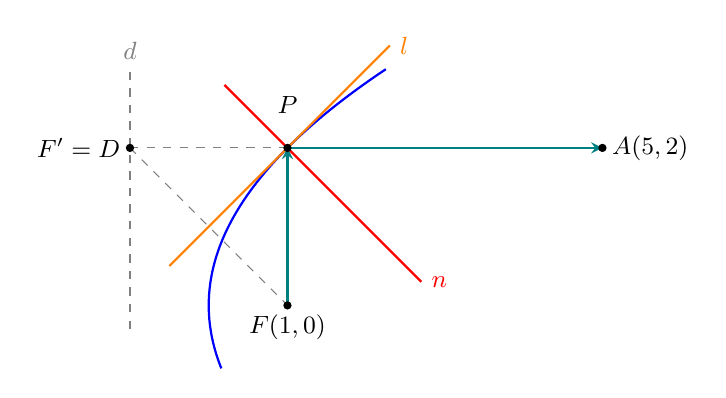
\begin{tikzpicture}[>=stealth,font=\small]
\draw[blue,thick,domain=-.8:3,samples=80] plot ({\x*\x/4},\x);
\draw[gray,dashed] (-1,-.3)--(-1,3) node[above] {$d$};
\draw[orange,thick] (-.5,.5)--(2.3,3.3) node[right] {$l$};
\draw[red,thick] (.2,2.8)--(2.7,.3) node[right] {$n$};
\draw[teal,thick,->] (1,0)--(1,2);
\draw[teal,thick,->] (1,2)--(5,2);
\draw[gray,dashed] (-1,2)--(1,2); \draw[gray,dashed] (-1,2)--(1,0);
\fill (1,0) circle(1.5pt) node[below] {$F(1,0)$};
\fill (1,2) circle(1.5pt); \node at (1,2.55) {$P$};
\fill (-1,2) circle(1.5pt) node[left] {$F'=D$};
\fill (5,2) circle(1.5pt) node[right] {$A(5,2)$};

\end{tikzpicture}
